\lecture{4}{16. September 2025}{Tvungen svingning af SDOF-systemer (del I)}

\begin{problem}{4.1}
  Bevis ved brug af ``ubestemte koefficienters''-metoden, at den partikulære løsning for et SDOF-system med masse $m$, dæmpning $c$ og stivhed $k$, der er påvirket af en harmonisk last med amplitude $F_0$ og frekvens $\Omega$, er givet ved
  \[ 
  d_{\mathrm{p}}(t) = \frac{F_0}{\sqrt{\left( k - m \Omega^2 \right)^2 + c^2 \Omega^2}} \cos \left( \Omega t - \tan^{-1} \left( \frac{c\Omega}{k - m\Omega^2} \right) \right)
  .\]
\end{problem}

\begin{derivation}
  Den generelle formel for tvungen svingning af et SDOF-system er
  \[ 
  m \ddot{d}(t) + c \dot{d}(t) + kd (t) = F (t) 
  .\]
  Fra ubestemte koefficienters metode har vi flg. partikulære løsning:
  \[ 
  d_p (t) = B_1 \cos \left( \Omega t \right) + B_2 \sin \left( \Omega t \right)
  .\]
  Ved indsættelse af den partikulære løsning og den drivende kraft $F = F_0 \cos \left( \Omega t \right)$ fås:
  \begin{align*}
    m &\left( - \Omega^2 B_1 \cos \left( \Omega t \right) - \Omega^2 B_2 \sin \left( \Omega t \right) \right) \\
    + c &\left( - \Omega B_1 \sin \left( \Omega t \right) + \Omega B_2 \cos \left( \Omega t \right) \right) \\
    + k &\left( B_1 \cos \left( \Omega t \right) + B_2 \sin \left( \Omega t \right) \right) = F_0 \cos \left( \Omega t \right) \\
    \implies \quad &\left( c \Omega B_2 + k B_1 - \Omega^2 m B_1 \right) \cos \left( \Omega t \right) \\
    + &\left( B_2 k - \Omega c B_1 - \Omega^2 m B_2 \right) \sin \left( \Omega t \right) = F_0 \cos \left( \Omega t \right)
  \end{align*}
  Vi lader nu $n \in \mathbb{N}_0$, da gælder at:
  \[ 
  \forall \Omega t = 2n \pi: \qquad \sin \left( \Omega t \right) = 0, \quad \cos \left( \Omega t \right) = 1
  .\]
  Da får vi ved indsættelse i udtrykket fra før:
  \begin{equation} \label{eq:41a}
    c \Omega B_2 + \left( k - \Omega^2 m \right) B_1 = F_0
  .\end{equation}
  Lader vi i stedet $m \in \mathbb{N}_0$, så:
  \[ 
  \forall \Omega t = 2m \pi + \frac{\pi}{2}: \qquad \sin \left( \Omega t \right) = 1, \quad \cos \left( \Omega t \right) = 0
  .\]
  Da får vi
  \begin{align}
    \left( k - \Omega^2 m \right)B_2 - \Omega c B_1 &= 0 \notag \\
    \implies \quad B_2 &= \frac{\Omega c B_1}{k - \Omega^2 m} \label{eq:41b}
  \end{align}
  Ved indsættelse af \Cref{eq:41b} i \Cref{eq:41a} fås:
  \begin{align*}
    \frac{\Omega^2 c^2 B_1}{k - \Omega^2 m} + \left( k - \Omega^2 m \right)B_1 &= F_0 \\
    \Omega^2 c^2 B_1 + \left( k - \Omega^2 m \right)^2 B_1 &= F_0 \left( k - \Omega^2 m \right) \\
    \left( \Omega^2 c^2 + \left( k - \Omega^2 m \right)^2 \right)B_{1} &= F_0 \left( k - \Omega^2 m \right) \\
    B_1 &= \frac{F_0 \left( k - \Omega^2 m \right)}{\Omega^2 c^2 + \left( k - \Omega^2 m \right)^2}
  .\end{align*}
  Fra \Cref{eq:41b} får vi da at
  \begin{align*}
    B_2 &= \frac{\Omega c F_0 \left( k - \Omega^2 m \right)}{\left( k - \Omega^2 m \right) \left( \Omega^2 c^2 + \left( k - \Omega^2 m \right)^2 \right)} \\
        &= \frac{\Omega c F_0}{\Omega^2 c^2 + \left( k - \Omega^2 m \right)^2}
  .\end{align*}
  Fra definitionen af $B \equiv \sqrt{B_1^2 + B_2^2}$ fås
  \begin{align*}
    B &= \sqrt{\left( \frac{F_0 \left( k - \Omega^2 m \right)}{\Omega^2 c^2 + \left( k - \Omega^2 m \right)^2} \right)^2 + \left( \frac{\Omega c F_0}{\Omega^2 c^2 + \left( k - \Omega^2 m \right)^2} \right)^2} \\
      &= \sqrt{\frac{F_0^2 \left( k - \Omega^2 m \right)^2}{\left( \Omega^2 c^2 + \left( k - \Omega^2 m \right)^2 \right)^2} + \frac{\Omega^2 c^2 F_0^2}{\left( \Omega^2 c^2 - \left( k - \Omega^2 m \right)^2 \right)^2}}\\
    &= \sqrt{\frac{F_0^2 \left( k - \Omega^2 m \right)^2 + \Omega^2 c^2 F_0^2}{\left( \Omega^2 c^2 + \left( k - \Omega^2 m \right)^2 \right)^2}} \\
    &= \sqrt{\frac{F_0^2 \left( \Omega^2 c^2 + \left( k - \Omega^2 m \right) \right)}{\left( \Omega^2 c^2 + \left( k - \Omega^2 m \right)^2 \right)^2}} \\
    &= \frac{F_0}{\sqrt{\Omega^2 c^2 + \left( k - \Omega^2 m \right)^2}}
  .\end{align*}
  Dermed er det vist at den rigtige faktor $B$ er angivet i opgaven.
  Nu mangler vi blot at vise at fasevinklen $\epsilon = \tan^{-1} \left( c \Omega / \left( k - m \Omega^2 \right) \right)$ også er korrekt.
  Denne er defineret som $\epsilon = \tan^{-1} \left( B_2 / B_1 \right)$.
  Ved indsættelse fås:
  \begin{align*}
  \epsilon &= \tan^{-1} \left( \frac{\Omega c F_0}{F_0 \left( k - \Omega^2 m \right)} \right) \\
           &= \tan^{-1} \left( \frac{\Omega c}{k - \Omega^2 m} \right)
  .\end{align*}
  Dermed er det vist.
\end{derivation}

\finalresult{
  \begin{aligned}
    B &= \frac{F_0}{\sqrt{\Omega^2 c^2 + \left( k - \Omega^2 m \right)^2}}  \\
    \epsilon &= \tan^{-1} \left( \frac{\Omega c}{k - \Omega^2 m} \right)
  .\end{aligned}
}


\begin{problemwithimage}{p4_2}{4.2}
    Vi returnerer til systemet behandlet i opgave 3.2 (se forrige lektion), som nu påføres en harmonisk last.
  Denne last er givet ved $F(t) = F_0 \cos \left( \Omega t \right)$, hvor $F_0 = \qty{1}{\kN}$, mens $\Omega$ ønskes bestemt. I denne forbindelse oplyses det, at fasevinklen i den stationære svingning er lig \ang{90}.
  a) Bestem lastfrekvensen, $\Omega$.
  b) Bestem flytningsamplituden i den stationære svingning, $B$.
  c) Bestem den dynamiske forstærkningsfaktor, $D$.
\end{problemwithimage}

\begin{derivation}
  Eftersom Fasevinklen i den stationære svingning er \ang{90} har vi $\tan \ang{90} \to \infty \implies p = 1 \implies \Omega = \omega_u = \qty{62,9}{\s^{-1}}$.

  Eftersom $p = 1$ har vi
  \begin{align*}
    D \equiv \frac{Bk}{F_0} &= \frac{1}{\sqrt{\left( 1 - p^2 \right)^2 + 4 \xi^2 p^2}} \\
                            &= \frac{1}{\sqrt{4 \xi^2}} \\
                            &= \frac{1}{2\xi} \\
    \implies \qquad B &= \frac{F_0}{2 \xi k_{\mathrm{eq}}}
  .\end{align*}
  Hvor $k_{\mathrm{eq}} = k_1 + k_2$ og $\xi$ er fundet/givet i opgave 3.2. Dermed er $D = \frac{1}{2\xi}$ også fundet.
\end{derivation}

\finalresult{
  \begin{aligned}
    \mathrm{a}) \quad \Omega &= \omega_u = \qty{62,9}{\s^{-1}} \\
    \mathrm{b}) \quad B &= \frac{F_0}{2\xi k_{\mathrm{eq}}} \\ 
    \mathrm{c}) \quad D &= \frac{1}{2\xi}
  .\end{aligned}
}


\begin{problem}{4.3}
  Bevis, at den styrende bevægelsesligning for SDOF-systemet skitseret på figur 3.6b i forelæsningsnoterne kan formuleres som
  \[ 
  \left( m + m_r \right) \ddot{d} (t) + c \dot{d}(t) + k d( t) = m_r \omega_r^2 e \sin \left( \omega_r t \right)
  .\]
\end{problem}

\begin{figure} [ht]
  \centering
  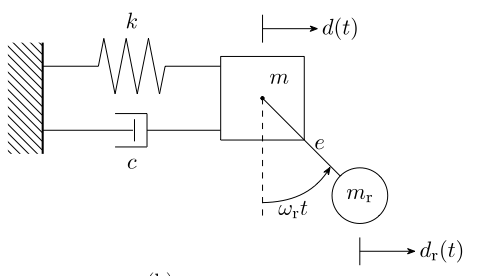
\includegraphics[width=0.5\linewidth]{./figures/p4_3.png}
  \caption{SDOF-systemet fra figur 3.6b i forelæsningen.}
  \label{fig:p4_3}
\end{figure}

\begin{derivation}
  Fra Newtons anden lov fås
  \[ 
  m \ddot{d}(t) + m_r \ddot{d}_r(t) = - c \dot{d}(t) - k d(t)
  .\]
  $d_r(t)$ kan også skrives som
  \[ 
  d_r(t) = d(t) + e \sin \left( \omega_r t \right)
  .\]
  Dermed har vi
  \[ 
  \ddot{d}_r(t) = \ddot{d}(t) - \omega_r^2 e \sin \left( \omega_r t \right)
  .\]
  Ved indsættelse af dette i Newtons 2. lov får vi
  \begin{align*}
    m \ddot{d}(t) + m_r \left( \ddot{d}(t) - \omega^2_r e \sin \left( \omega_r t \right) \right) + c \dot{d}(t) + kd(t) &= 0 \\
    \left( m + m_r \right) \ddot{d}(t) + c \dot{d}(t) + kd(t) &= m_r \omega^2_r e \sin \left( \omega_r t \right)
  .\end{align*}
\end{derivation}

\finalresult{(m + m_r) \ddot{d}(t) + c \dot{d}(t) + kd(t) = m_r \omega_r^2 e \sin \left( \omega_r t \right)}

\begin{problemwithimage}{p4_4}{4.4}
  Vi betragter det skitserede pendulsystem og antager, at stangen er uendelig stiv, uniform, masseløs og uden dæmpning.
  En bevægelig understøtning virker, som skitseret, med $\eta(t) = \eta_0 \cos \left( \omega_b t \right)$.
  Systemet skal modelleres som et SDOF-system med frihedsgraden værende rotation af stangen, $\theta(t)$.
  a) Udled bevægelsesligningen for $\theta (t)$ under antagelsen om LTI-betingelser.
  b) Bestem (symbolsk) den udæmpede vinkelegenfrekvens, $\omega_u$.
\end{problemwithimage}

\begin{derivation}
  Momentet omkring stangen (idet den roteres en lille vinkel $\theta$ væk fra fjederen) giver
  \[ 
  I \ddot{\theta} = - k \left( L \sin \theta - \eta \right)L \cos \theta - mg L \sin \theta
  .\]
  Vi bruger $\cos \theta \approx 1$ og $\sin \theta \approx \theta$ og får
  \[ 
    I \ddot{ \theta} = - k \left( L \theta - \eta \right) L - mgL \theta
  .\]
  $\eta (t) = \eta_0 \cos \left( \omega_b t \right)$ er givet i opgaven, hvorfor
  \begin{align*}
    I \ddot{ \theta} &= - k \left( L \theta - \eta_0 \cos \left( \omega_b t \right) \right) L - mgL \theta \\
    I \ddot{ \theta} + \left( k L^2 + mgL \right) \theta &= kL \eta_0 \cos \left( \omega_b t \right)
  .\end{align*}
  For en stiv stang der roterer om enden er $I = m L^2$ og vi får derfor
  \[ 
  m L^2 \ddot{\theta} + \left( kL^2 + mgL \right)\theta = kL \eta_0 \cos \left( \omega_b t \right)
  .\]
  
  For at bestemme den udæmpede vinkelegenfrekvens bruger vi blot
  \begin{align*}
    \omega_u &= \sqrt{\frac{B_2}{B_1}} \\
             &= \sqrt{\frac{k L^2 + mgL}{mL^2}} \\
             &= \sqrt{\frac{kL + mg}{mL}}
  .\end{align*}
\end{derivation}

\finalresult{
  \begin{aligned}
    \mathrm{a}) &\quad m L^2 \ddot{\theta} + \left( k L^2 + mgL \right)\theta = k L \eta_0 \cos \left( \omega_b t \right) \\
    \mathrm{b}) &\quad \omega_u = \sqrt{\frac{k L + mg}{mL}}
  .\end{aligned}
}
